\chapter{Planning}
\label{chap:planning}
An initial planning for the research is made and shown in figure \ref{fig:gantt_planning}. This planning is open to changes and is mostly created to provide a clearer picture of the research. It should be noted that the overall project goals set out in this document are optimistic and it should be expected that not all of them will be achieved. Buffer time is included within the set times. An expectation that during the course of the PhD, more responsibilities outside of personal research will be taken on. This results in less time per week being spent on personal research and thus more time is planned. 
%\par 
%The adaptation of the flume tank is expected to take up time, especially since the tank is not available from February till April. During this time the experiments into air entrapment will be designed and conducted. 
\begin{figure}[]
	\centering
	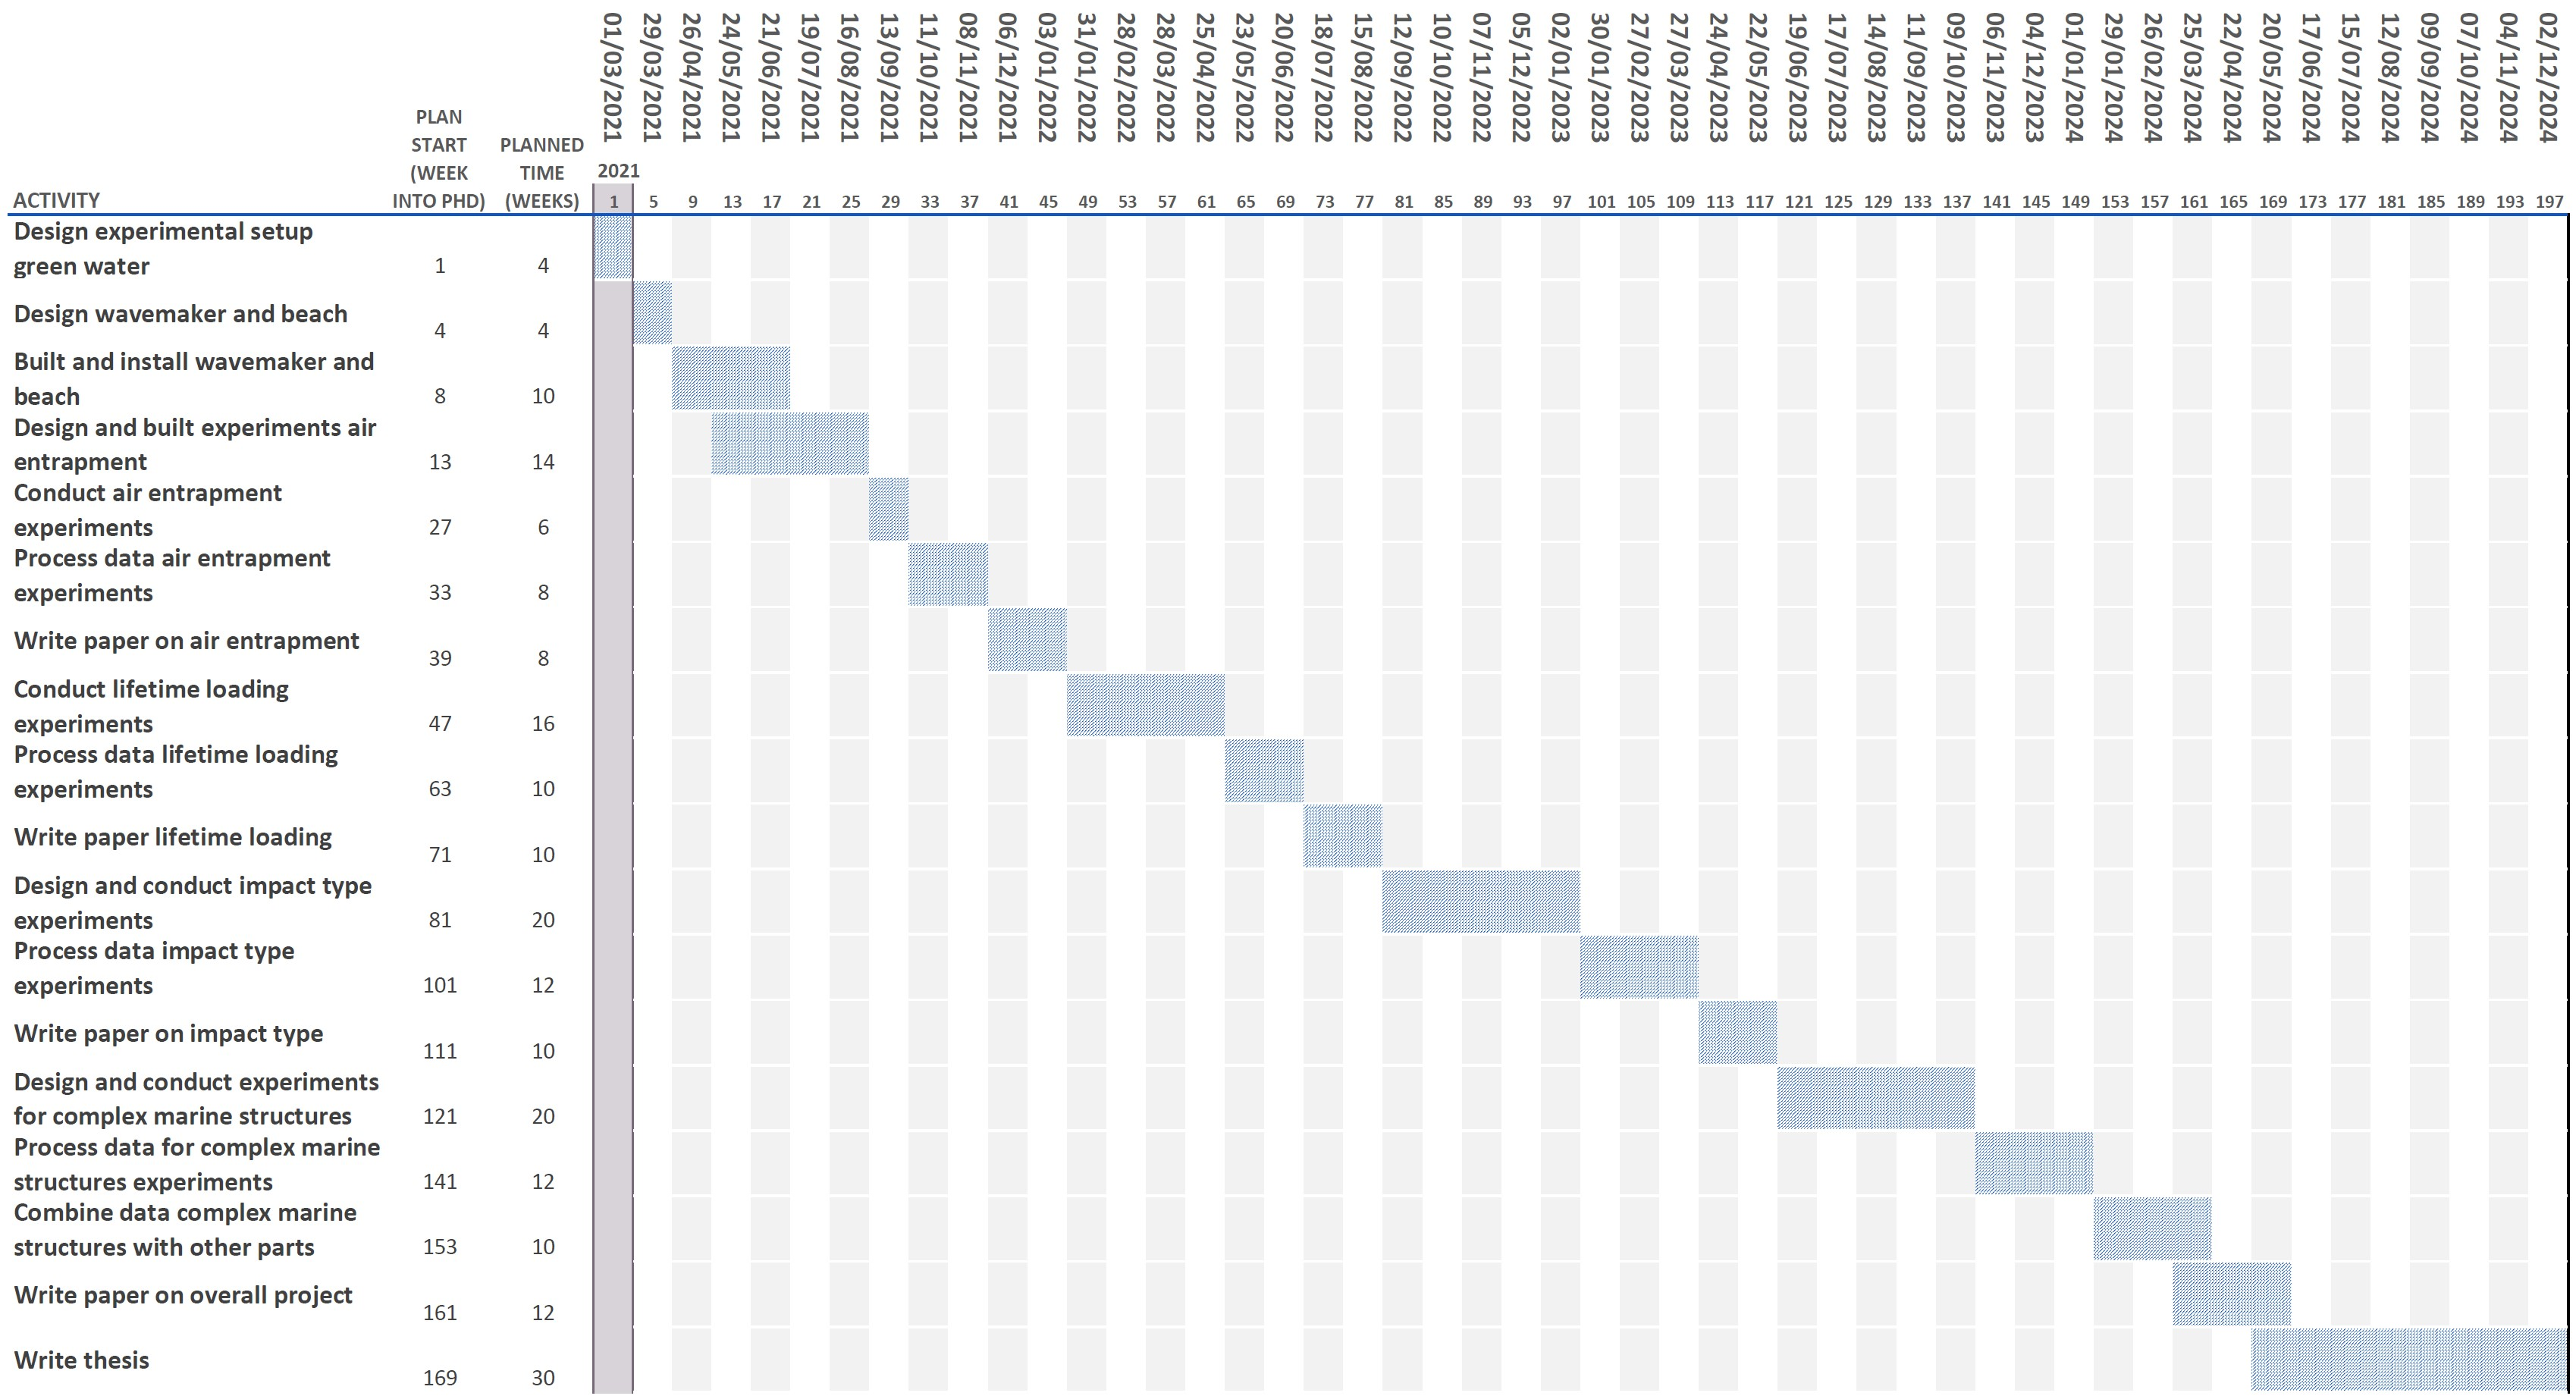
\includegraphics[width=1.8\linewidth, angle =90]{figs/GanttPlanning.jpg}
	\caption{Gantt planning for the research project}
	\label{fig:gantt_planning}
\end{figure}

\section{PhD agreement}
\label{sec:phd_agreement}
In the document ('PhD Agreement') the goals for the PhD are set out. In this paragraph these goals are further clarified.
\par 
For official documentation achievable goals need to be set and agreed to. As stated in the previous paragraph, the research objectives set out within this document are optimistic. In agreement with the daily supervisor P.R. Wellens a publication goal of three papers is set. The planning is to have an outline of a first paper by the Go/No-Go meeting, which will be planned before December 1\(^{st}\) of 2021. 
\par 
The required educational activities are expected to come into focus after the first year of the project, but this could be sooner depending on the circumstances. The first educational 
activity will probably be supervising a master thesis. 
\par 
During the PhD, graduate school credits should be obtained. There are three topics: discipline related skill, transferable skills and research skills, with a minimum of 15 graduate school credits per topic. Improving discipline related skills early in the project is thought to benefit the final results, and thus in the first year a focus is put on developing these skills. Some courses for transferable skills and research skills will be followed to develop these skill further as well. The goal is to have obtained over 20 graduate school points before the Go/No-Go meeting.